\documentclass[conference,letterpaper]{IEEEtran}
\IEEEoverridecommandlockouts
\usepackage{graphicx}
\usepackage{booktabs}
\usepackage{tabularx}
\usepackage{array}
\usepackage{url}
\usepackage{cite}
\usepackage[hidelinks]{hyperref}
\hypersetup{pdfauthor={Paphanin Amnuaikitwanit; Thepchai Supnithi; Nongnuch Ketui}}
\usepackage{microtype}
\pdfminorversion=7

\title{ThaiVoice-GUIBench: A Controlled Diagnostic Benchmark for Thai and Code-Switched Spoken GUI Grounding}
\author{\IEEEauthorblockN{Paphanin Amnuaikitwanit, Thepchai Supnithi, and Nongnuch Ketui}}

\begin{document}
\IEEEpubid{\makebox[\columnwidth][l]{979-8-3195-1044-0/26/\$31.00 \textcopyright2026 IEEE}\hspace{\columnsep}\makebox[\columnwidth]{}}
\maketitle
\begin{abstract}
We present ThaiVoice-GUIBench, a small diagnostic benchmark for Thai and Thai--English spoken GUI grounding, with 20 synthetic screens, 128 commands, and 480 TTS audio files, of which 471 pass the audio audit. Commands cover verbatim labels, paraphrases, intents, and visual/positional references. All 18 code-switched commands are verbatim (T1), so code-switching coverage is preliminary. Whisper large-v3 has lower character and Thai-tokenized word error rates than Typhoon ASR on this audio. GPT-5.5 click accuracy is 76.56 percent on gold text, 75.80 on Whisper, and 76.43 on Typhoon transcripts; command-clustered intervals show no detectable gold-versus-ASR difference. Three frozen correction methods yield no clear evidence of improved click accuracy under this protocol. An adverse changed-subset difference occurs in one exploratory comparison, but raw and corrected predictions were collected in independent runs. Identical-prompt UI-TARS reruns change click correctness on 25--27 percent of items. Changed/unchanged subsets and no-op controls expose this confounding without isolating correction causality. The benchmark supports separate reporting of transcript recovery, false correction, and downstream click outcomes.
\end{abstract}

\begin{IEEEkeywords}
Thai speech recognition, GUI grounding, code-switching, transcript correction.
\end{IEEEkeywords}
\section{Introduction}

Spoken interaction with graphical interfaces combines automatic speech recognition (ASR) with visual grounding: the system must recover a command and locate its intended control. Thai commands may mix Thai syntax with English screen labels, paraphrase a label, describe an intent, or refer to a visual position. A small transcript error may remove a useful screen anchor, while visual context may still support a correct click.

ThaiVoice-GUIBench makes these outcomes inspectable in a fixed single-click task. It contains 20 synthetic mobile-style screens and TTS speech, rather than production interfaces or real-speaker recordings. Four command tiers distinguish verbatim labels, paraphrases, intents, and visual/positional references. We compare two ASR systems and two grounding models, then evaluate three fixed-rule transcript corrections; the release includes the pipeline diagram. Grounding prompts receive the screenshot and command, without the target identifier, target box, gold answer, or candidate list.

Correction is evaluated at both transcript and click levels. Visible screen strings may help recover a label but may also inject unsupported content. Moreover, raw and corrected grounding were run independently, days apart. A changed click can therefore reflect rerun variability as well as changed text. Changed/unchanged subsets and no-op controls reveal this attribution problem; they do not solve it.

We ask how ASR errors vary by tier and TTS condition, whether raw-ASR grounding differs detectably from gold-text grounding, and when transcript changes coincide with better or worse clicks. Our contributions are an auditable Thai diagnostic resource, tiered evaluation that retains parse and out-of-bounds failures, three frozen correction baselines with benefit-and-harm reporting, and analyses exposing rerun confounding. The results support diagnosis within this synthetic benchmark, without establishing effects for real users or broader code-switching patterns.

\section{Related Work}
\IEEEpubidadjcol

\paragraph{Multilingual and Thai ASR}
Large multilingual ASR systems provide practical baselines across languages and acoustic conditions \cite{radford2023whisper,fasterwhisper}. Code-switched ASR remains data-scarce and difficult even when multilingual resources are transferred \cite{winata2020codeswitch}. Thai research distinguishes English code-mixing from established borrowing \cite{rungrojsuwan2023mixing}, and loanwords may undergo systematic phonological adaptation \cite{kenstowicz2006thai}. Because Thai spaces do not consistently delimit words, we pair character error rate with Thai-tokenized word error rate using PyThaiNLP \cite{pythainlp}, and separately track English loanwords. Our TTS diagnostic is not a substitute for a real Thai--English code-switched speech corpus.

\paragraph{Spoken interaction and GUI grounding}
Spoken assistants have used graphical feedback to expose incremental understanding \cite{kennington2016spoken}; more recent speech-driven GUI agents consume audio and screenshots directly for grounding and planning \cite{han2025guirobotron}. In parallel, visual UI grounding maps free-form language and screenshots to interface elements \cite{qian2024visual}, while UI-TARS extends screenshot-based grounding toward native GUI action models \cite{uitars}. We instead isolate one coordinate prediction in a cascaded TTS--ASR pipeline. This narrow protocol makes transcript errors, target containment, parse failure, and out-of-bounds behavior directly measurable.

\paragraph{Context-aware transcript correction}
Downstream context can constrain ASR correction, and visible interface strings provide a compact domain lexicon. That context is also risky: matching a plausible screen label can alter an already adequate transcript or inject a label unsupported by an intent-level command. We treat screen-aware correction as a fixed intervention rather than a learned component, report recovery together with false-correction rate, and report changed-text associations alongside unchanged-prompt variability without isolating causality.

\section{Benchmark Design}

\subsection{Task, synthetic screens, and targets}

The benchmark input is one spoken command and a screenshot; the evaluated cascade transcribes the audio before predicting a single click $(x,y)$ in screenshot pixels, with the origin at the upper-left. Evaluation checks image bounds and containment in the gold target box. The predicted element is derived after inference as the smallest annotated box containing the point. Unparseable outputs and out-of-bounds points count as incorrect in the primary denominator. No navigation sequence or autonomous recovery is evaluated.

The frozen dataset contains 20 synthetic mobile-style screens, five each for messaging, mock finance, settings, and shopping (Table~\ref{tab:dataset}). Each screen includes visible labels, a screen lexicon, clickable boxes, and confusable distractors. Screens contain no real institutions, credentials, private accounts, or user data. Thirty-two explicit intent--screen mappings define the targets; target identifiers, boxes, distractor IDs, and candidate lists are excluded from grounding prompts.

\begin{table}[t]
\centering
\caption{Frozen dataset statistics.}
\label{tab:dataset}
\small
\begin{tabular}{lr}
\toprule
Statistic & Count \\
\midrule
Screens (4 domains) & 20 \\
Intent--screen mappings & 32 \\
Commands (32 per tier) & 128 \\
Pure Thai / code-switched & 110 / 18 \\
Commands with loanwords & 18 \\
Audio manifest rows & 480 \\
OpenAI / Azure audio & 256 / 224 \\
Valid / excluded audio & 471 / 9 \\
\bottomrule
\end{tabular}
\end{table}


\subsection{Command construction and validation}

Deterministic templates (seed 42) generate one command per mapping and tier. \textbf{T1 verbatim} may use the visible target label; \textbf{T2 paraphrase} uses a synonym or translation; \textbf{T3 intent} describes the desired outcome; and \textbf{T4 visual/positional} uses appearance or location. T2/T3 use intent-specific templates and T4 uses screen geometry and visual attributes rather than target-label wording. Automated anti-circularity checks reject target labels and listed copied-label aliases in T2--T4. These checks address lexical leakage, not naturalness or unambiguous interpretation.

One Thai-speaking author created and reviewed the Thai templates and checked all 128 commands for naturalness and ambiguity, alongside the recorded tier, leakage, and ASR/TTS-risk checks. The audit scaffold heuristically prefilled naturalness as slightly awkward when a command contained the mock-domain qualifier and natural otherwise; these initial scores were not independent human ratings. The review records contain 20 stylistic edits and no removals. The recorded edits simplify wording, including removal of the mock-domain qualifier. Author review is not an independent human target-selection study, and residual ambiguity remains possible.

There are 32 commands per tier, 110 pure-Thai and 18 code-switched commands. All code-switched commands are T1. Language and tier effects therefore cannot be separated, and this subset is preliminary coverage rather than a representative sample of Thai--English code-switching.

\subsection{TTS audio and weighting}

All speech is synthetic. Two OpenAI voices cover all 128 commands (256 files); Azure's first voice covers all commands and its second covers only the 96 test commands (224 files). Thus 32 dev commands have three renditions and 96 test commands have four before exclusions. The 18 code-switched commands have 70 renditions: two dev commands have three each and 16 test commands have four each. Of 480 files, 471 pass the audit. All nine exclusions are Azure code-switched T1 renditions, leaving 61 valid code-switched files. This selective exclusion may make code-switched ASR results optimistic.

Primary ASR and raw/corrected click aggregates weight valid audio files equally, so commands with more retained renditions receive more weight. Gold-text grounding uses one prediction per command; the paired bootstrap described below averages audio renditions within command. The manifest preserves command, tier, language, provider, voice, split, and exclusion provenance. Corrected variants leave screenshots, targets, and original ASR records unchanged.

\section{Method}

\subsection{ASR and grounding baselines}

We compare Whisper large-v3 through faster-whisper v1.2.1~\cite{radford2023whisper,fasterwhisper} and hosted \texttt{typhoon-asr-realtime} through the provider's \texttt{/v1} transcription API~\cite{opentyphoon}. Metrics are whitespace-normalized character error rate (CER), Thai-tokenized word error rate (WER) with PyThaiNLP v5.3.4~\cite{pythainlp}, literal loanword error rate (LER), and ASR failure rate. LER checks annotated Latin-form loanwords; it does not establish semantic equivalence between Thai transliterations and Latin spellings.

The hosted grounder is GPT-5.5 through the Responses API \texttt{/v1/responses}, Python SDK v2.44.0; saved responses resolve the alias to \texttt{gpt-5.5-2026-04-23}~\cite{openaiapi}. The local grounder is UI-TARS-1.5-7B~\cite{uitars}, abbreviated UI-TARS, served through vLLM in bfloat16. Both receive one screenshot, the transcript, image dimensions, pixel-coordinate conventions, and a single-click request, using model-specific wording and a shared JSON output schema. Numeric coordinates must parse; parse success alone does not imply a valid or correct click. Exact prompts, available configurations, and raw responses are retained in the reproducibility package.

\subsection{Frozen correction interventions}

Parameters and aliases were frozen before final correction evaluation, without tuning to the final results. \textbf{A: no-screen cleanup} normalizes Unicode, whitespace, and punctuation. \textbf{B: screen string matching} uses conservative exact or near-exact visible-label matches. \textbf{C: screen-aware alias correction} additionally uses fixed Thai meanings, phonetic forms, and Latin-normalized aliases. Fixed string-similarity thresholds for B/C are 0.95/0.94 and minimum confidences are 0.94/0.93; the full rules and alias inventory are supplied with the package.

Correction may use the ASR text, screen ID, visible-screen lexicon, and frozen alias table, but not targets, gold text, distractor lists, or grounding outcomes. Uncertain matches preserve the input. T3/T4 label replacement requires an existing matching surface form. Accepted changes record their spans, matched label, score, confidence, and reason.

\subsection{Transcript metrics and attribution boundary}

Literal recovery means lower CER or fewer annotated loanword errors. Literal false correction means higher CER, or any change when raw ASR exactly matches gold. These are string-based criteria, not judgments of linguistic harm. In an additional post-hoc diagnostic, a change is cosmetic if raw and corrected text become identical after NFKC and whitespace normalization. Remaining changes are non-cosmetic under that rule; normalized CER then supplies separate recovery and false-correction counts. This does not equate every non-cosmetic edit with a semantic error.

Raw grounding was collected July 9--11, 2026, and corrected grounding July 18--19. No inference wrapper set a deterministic seed or explicit temperature. Unchanged/no-op comparisons expose differences possible without textual edits; changed-subset comparisons remain confounded by independent inference. Directional shifts alone do not establish execution-environment drift.

\section{Experiments and Results}

\subsection{Protocol and exploratory statistics}

ASR and audio-conditioned grounding use all 471 valid files. Parse failures and out-of-bounds coordinates remain incorrect. Click transitions are CC (both correct), WC (raw wrong, corrected-run correct), CW (raw correct, corrected-run wrong), and WW (both wrong). Frozen counts are primary. Exact two-sided sign tests on WC/CW, Wilson intervals, command-clustered bootstraps, and identical-prompt UI-TARS reruns were added post hoc. The reported sign-test $p$-values are exploratory, unadjusted for multiple comparisons, and calculated at audio-item level despite repeated renditions per command; they do not establish confirmatory or causal effects.

\subsection{ASR performance}

Both ASR systems return records for all 471 files (Table~\ref{tab:asr}). Whisper has lower CER/WER on this audio. Code-switched CER is 10.02 percent for Whisper and 22.03 for Typhoon. Literal LER is 45.90 percent (28/61 audio-level instances) and 96.72 percent (59/61), respectively. These 61 instances derive from only 18 commands. Equivalent Thai-script transliterations may contribute to literal LER, but that explanation has not been established by an exhaustive lexical audit; lexical errors, script differences, and omissions have not been separated.

\begin{table}[t]
\centering
\caption{ASR performance (percent; $n=471$ each). LER is over 61 audio-level loanword instances.}
\label{tab:asr}
\small
\begin{tabular}{lrrrr}
\toprule
ASR & CER & WER & LER & Fail \\
\midrule
Whisper large-v3 & 5.55 & 10.72 & 45.90 & 0.00 \\
Typhoon ASR & 6.95 & 13.27 & 96.72 & 0.00 \\
\bottomrule
\end{tabular}
\end{table}


\subsection{Gold text versus raw ASR}

GPT-5.5 parses every baseline output, with pooled click accuracy of 76.56 percent on gold, 75.80 on Whisper, and 76.43 on Typhoon text (Table~\ref{tab:grounding}). UI-TARS scores 44.53/39.07/40.34 percent and has 9/34/29 parse failures, respectively. Its pooled point-in-image rates remain below 92 percent. Gold accuracy is reported separately by tier: GPT-5.5 T4 is 62.50 percent, whereas its raw-ASR T4 scores are 58.33--59.17 percent. Neither value establishes a model ceiling.

Gold uses 128 commands and ASR conditions use 471 correlated renditions. Existing paired bootstraps average ASR click correctness within command, subtract that command's gold score, and resample 128 commands (10,000 draws; seed 20260719). The GPT-5.5 Whisper/Typhoon mean differences are $-0.52$/$+0.07$ points, with 95 percent intervals $[-3.12,+2.02]$/$[-2.34,+2.86]$; UI-TARS differences are $-4.43$/$-3.32$, with intervals $[-12.50,+3.71]$/$[-10.87,+4.36]$. There is no detectable gold-versus-ASR difference. Small underlying effects, robustness to ASR errors, and insufficient benchmark sensitivity or power remain possible.

\begin{table*}[t]
\centering
\caption{Baseline grounding (percent). Click includes failures; PFail is parse-failure rate. Gold has 32 commands per tier; each ASR condition has 111 T1 and 120 T2--T4 audio items. Tier scores are condition-specific, not model ceilings.}
\label{tab:grounding}
\small
\begin{tabular}{llrrrrrrr}
\toprule
Model & Transcript & $n$ & Click & PFail & T1 & T2 & T3 & T4 \\
\midrule
GPT-5.5 & Gold & 128 & 76.56 & 0.00 & 100.00 & 71.88 & 71.88 & 62.50 \\
GPT-5.5 & Whisper & 471 & 75.80 & 0.00 & 100.00 & 73.33 & 72.50 & 59.17 \\
GPT-5.5 & Typhoon & 471 & 76.43 & 0.00 & 100.00 & 75.83 & 73.33 & 58.33 \\
UI-TARS & Gold & 128 & 44.53 & 7.03 & 75.00 & 34.38 & 43.75 & 25.00 \\
UI-TARS & Whisper & 471 & 39.07 & 7.22 & 70.27 & 29.17 & 29.17 & 30.00 \\
UI-TARS & Typhoon & 471 & 40.34 & 6.16 & 56.76 & 41.67 & 40.83 & 23.33 \\
\bottomrule
\end{tabular}
\end{table*}


\subsection{Transcript changes and pooled clicks}

Table~\ref{tab:correction} separates literal transcript metrics from observed pooled click differences. Typhoon A/B are complete no-op controls. Under the post-hoc normalization rule, all 72 Whisper A changes and 63 of 72 B changes are cosmetic. B has nine normalized-CER recoveries and no normalized false corrections. C has 38 Whisper and 48 Typhoon normalized false corrections. Thus large literal A/B false-correction rates mostly reflect normalization mismatch; normalized counts also remain metric-based, rather than direct semantic-error rates.

Pooled click differences are mixed and mostly negative, but independent reruns prevent causal attribution to correction. In particular, the UI-TARS/Typhoon/A no-op differs by $-6.16$ points despite identical transcript text. Figure~\ref{fig:correction-tier} retains the tier variation and negative differences; its literal FCR must be interpreted alongside the cosmetic-change diagnostic.

\begin{table*}[t]
\centering
\caption{Literal transcript metrics (percent; shared across grounders) and observed pooled click differences (percentage points). FCR includes cosmetic changes; net is recovery count minus false-correction count. Click differences compare independent runs. W/T denote Whisper/Typhoon.}
\label{tab:correction}
\small
\begin{tabular}{llrrrrrr}
\toprule
ASR & Method & Changed & Recovery & FCR & Net & GPT-5.5 $\Delta$ & UI-TARS $\Delta$ \\
\midrule
W & A & 15.29 & 0.00 & 15.29 & -72 & -0.64 & +0.21 \\
W & B & 15.29 & 0.64 & 15.29 & -69 & -0.42 & -1.70 \\
W & C & 23.99 & 1.70 & 23.35 & -102 & -1.91 & -4.03 \\
T & A & 0.00 & 0.00 & 0.00 & 0 & -1.27 & -6.16 \\
T & B & 0.00 & 0.00 & 0.00 & 0 & -0.85 & -0.21 \\
T & C & 11.25 & 3.18 & 10.19 & -33 & -1.27 & -1.49 \\
\bottomrule
\end{tabular}
\end{table*}


\begin{figure*}[t]
    \centering
    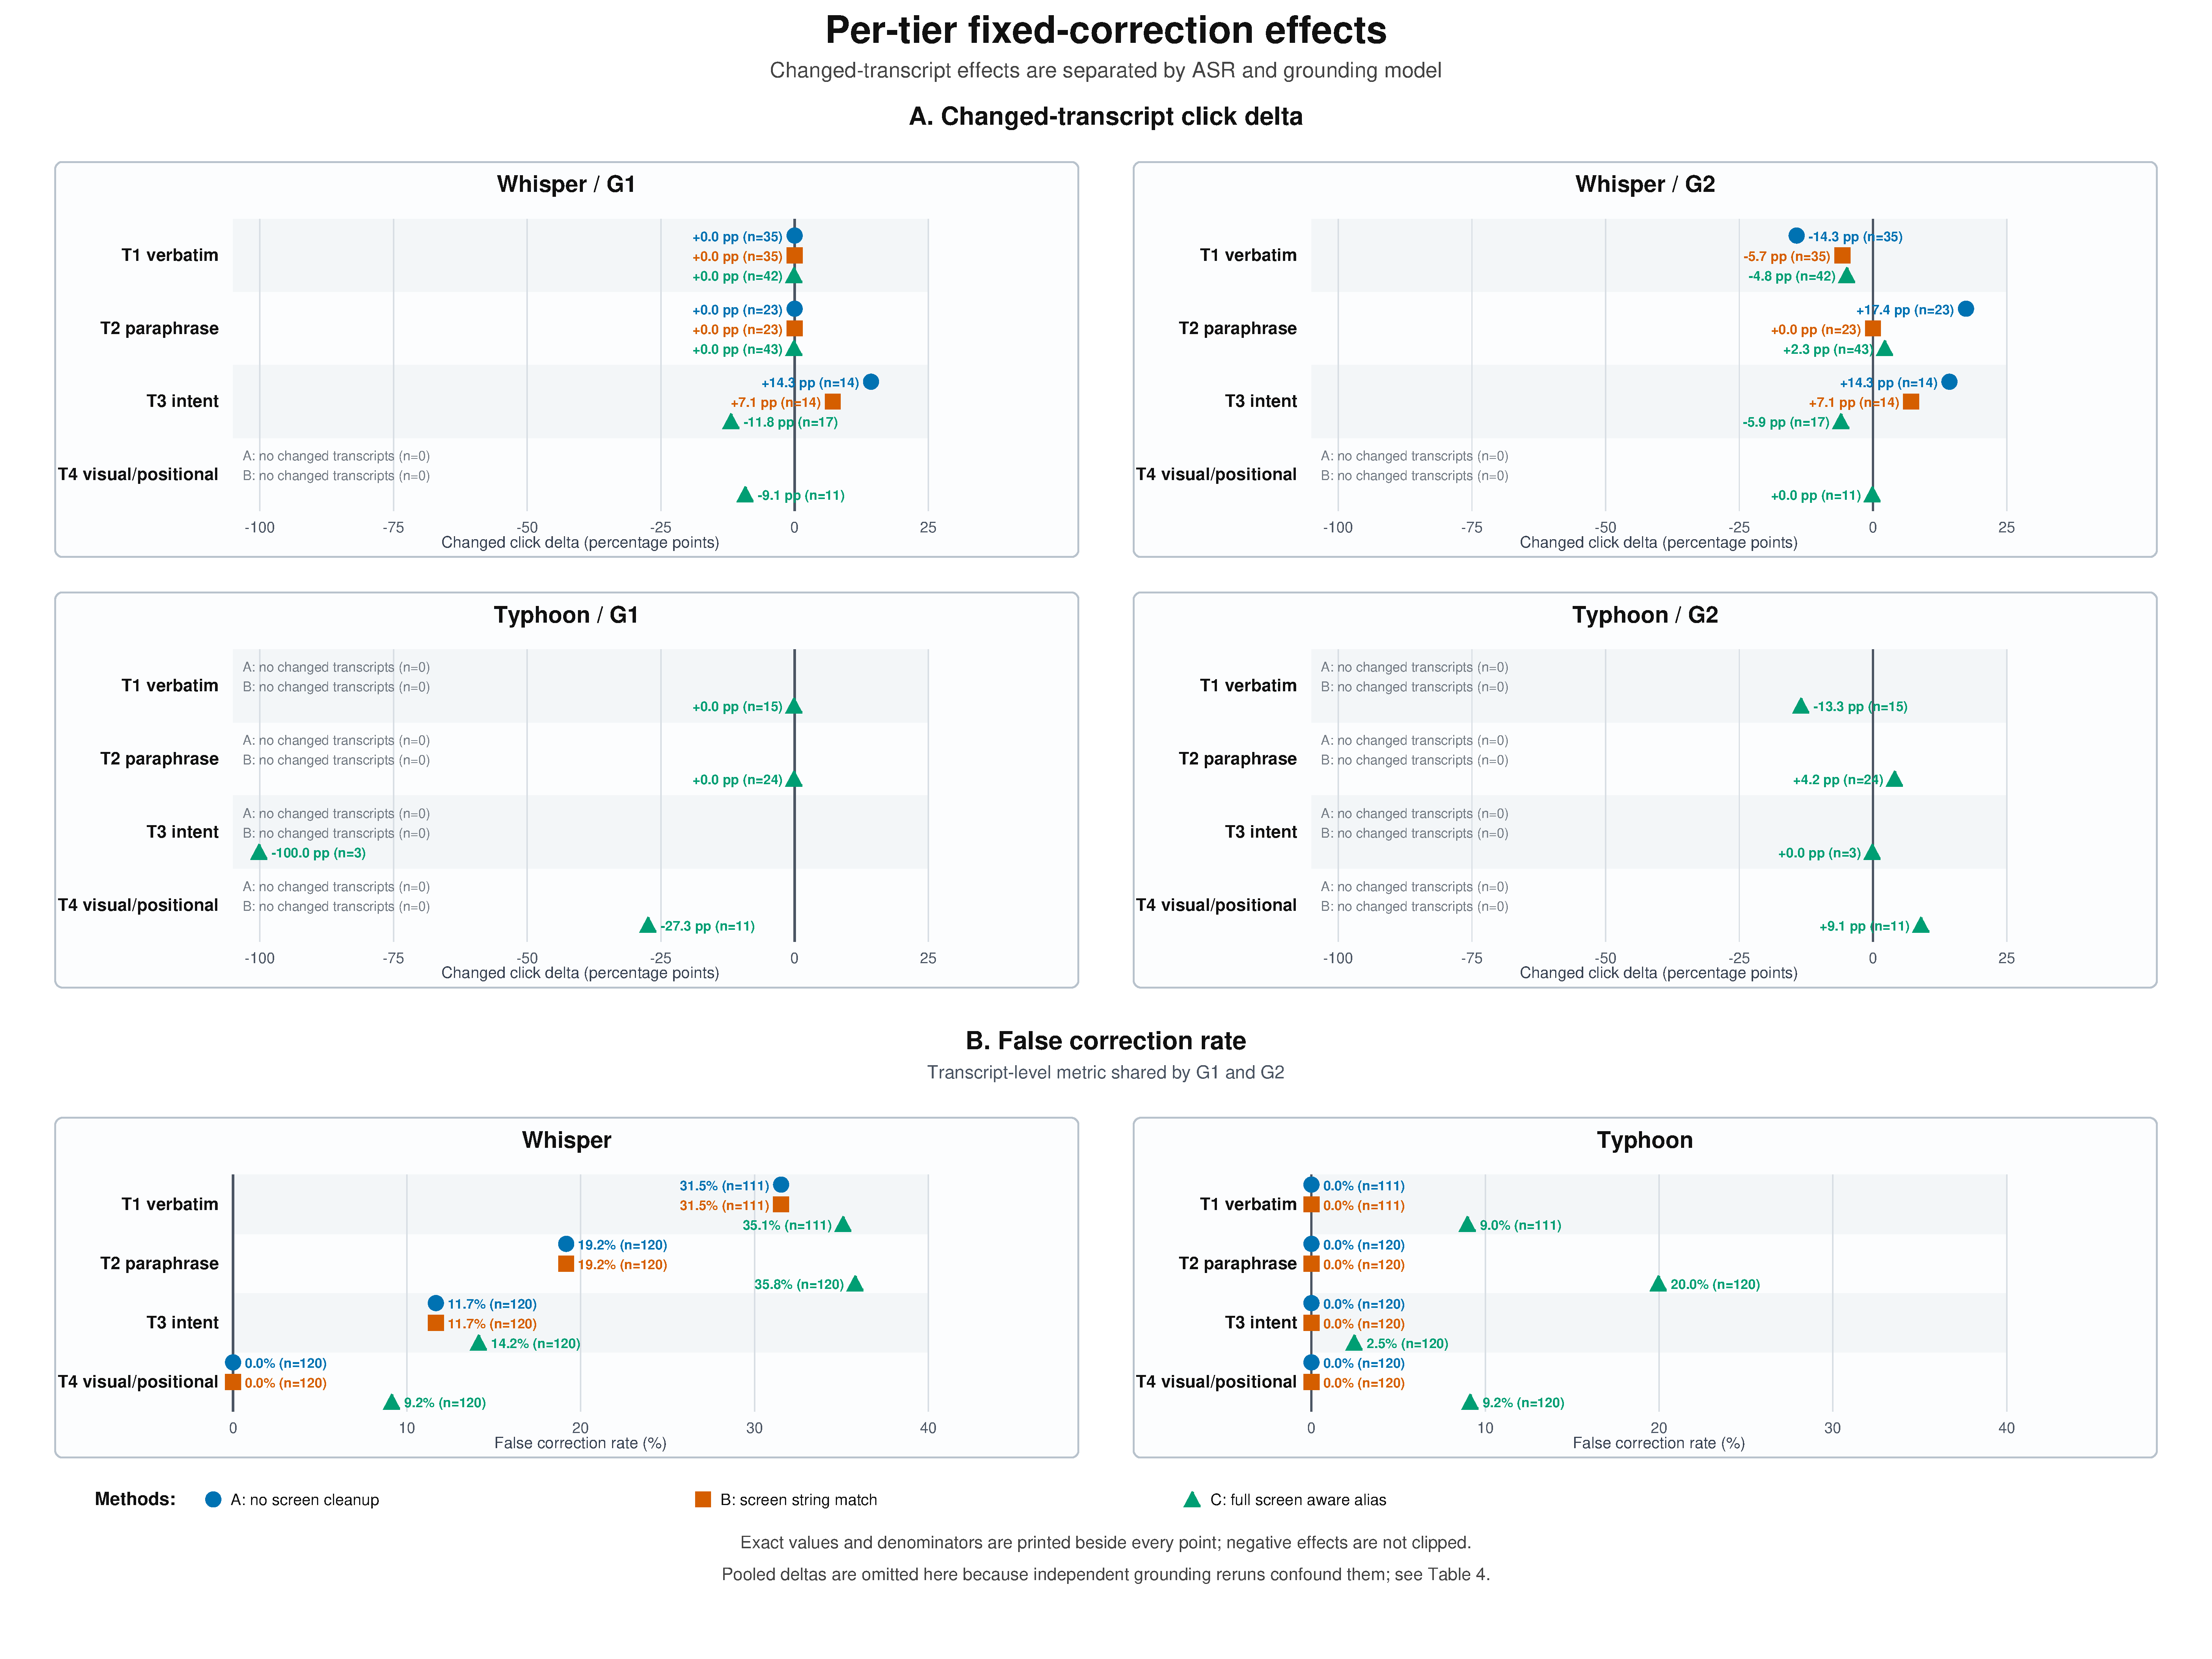
\includegraphics[width=\textwidth]{figures/figure2_per_tier_correction_effects.pdf}
    \caption{Observed per-tier changed-transcript click differences and literal false-correction rate (FCR), using the frozen figure data. Artwork uses ``effects'' for cross-run differences, not causal estimates. FCR is string-based and includes cosmetic changes. Table~\ref{tab:changed-unchanged} reports unchanged/no-op comparisons. G1/G2 denote GPT-5.5/UI-TARS.}
    \label{fig:correction-tier}
\end{figure*}

\subsection{Changed, unchanged, and rerun comparisons}

For GPT-5.5/Whisper, A/B changed-subset differences of $+2.78$/$+1.39$ points reflect only two/one net WC flips (exploratory $p=0.50/1.0$; Table~\ref{tab:changed-unchanged}). GPT-5.5/Typhoon/C shows an adverse difference in one exploratory comparison: $-11.32$ points among 53 changed items, WC=0 and CW=6, with unadjusted post-hoc $p=0.03125$. The six deteriorations arise from \emph{three unique commands}, not six independent commands. Repeated renditions, multiple testing, and separate inference runs preclude a general claim that C degrades performance. GPT-5.5/Whisper/C differs by $-2.65$ points ($p=0.375$).

UI-TARS changed-subset WC/CW counts are nearly balanced. Its Typhoon/A no-op has WC=49 and CW=78 ($p=0.0127$, subject to the same exploratory caveats). The existing identical-prompt rerun of all three raw UI-TARS conditions changes click correctness on 25--27 percent of items and parse status on 10--11 percent. Exact coordinates recur for only 1--5 items per condition. Net gold/Whisper/Typhoon differences are $+3.13$/$+0.21$/$-0.64$ points. These records demonstrate rerun variability but neither remove it from corrected-versus-raw comparisons nor establish serving-system drift.

\begin{table*}[t]
\centering
\caption{Observed changed versus unchanged click differences. Independent runs do not isolate correction causality. Deltas are percentage points. Same-U is exact coordinate repeatability among unchanged prompts. A dash means no transcript changed.}
\label{tab:changed-unchanged}
\small
\begin{tabular}{lllrrrrr}
\toprule
Grounding & ASR & Method & $n_C$ & $\Delta_C$ & $n_U$ & $\Delta_U$ & Same-U \\
\midrule
GPT-5.5 & W & A & 72 & +2.78 & 399 & -1.25 & 279/399 \\
GPT-5.5 & W & B & 72 & +1.39 & 399 & -0.75 & 277/399 \\
GPT-5.5 & W & C & 113 & -2.65 & 358 & -1.68 & 247/358 \\
GPT-5.5 & T & A & 0 & -- & 471 & -1.27 & 333/471 \\
GPT-5.5 & T & B & 0 & -- & 471 & -0.85 & 332/471 \\
GPT-5.5 & T & C & 53 & -11.32 & 418 & 0.00 & 278/418 \\
UI-TARS & W & A & 72 & +1.39 & 399 & 0.00 & 5/399 \\
UI-TARS & W & B & 72 & -1.39 & 399 & -1.75 & 3/399 \\
UI-TARS & W & C & 113 & -1.77 & 358 & -4.75 & 1/358 \\
UI-TARS & T & A & 0 & -- & 471 & -6.16 & 2/471 \\
UI-TARS & T & B & 0 & -- & 471 & -0.21 & 5/471 \\
UI-TARS & T & C & 53 & 0.00 & 418 & -1.67 & 4/418 \\
\bottomrule
\end{tabular}
\end{table*}


\subsection{Manual review and qualitative cases}

One human reviewer coded 140 deterministically selected cases using the saved review guide. Selection covered failures, correction transitions, no-op changes, loanwords, and T3/T4 difficulties, then balanced tier and model/method groups; each tier contributes 35 cases. This is a purposive stratified sample, not a prevalence sample. The reviewer saw system identities, gold targets/text, automatic candidate categories, predicted coordinates, and click outcomes. Coding was unblinded and assigned one final category with evidence notes per case. Inter-reviewer agreement was not measured; between-reviewer disagreement resolution was inapplicable.

The guide includes lexical/segmentation errors, confusable labels, visual/positional failures, ambiguity, over-correction, parse/out-of-bounds failures, transcript/click transitions, and unchanged-prompt variability. The largest sampled categories are variability (27), confusable labels (16), positional failures (16), parse failures (15), and ambiguous instructions (14). These counts cannot estimate benchmark-wide ambiguity or identify its contribution to total error.

Case 093 (shopping\_002, T2) replaces a Thai basket expression with \emph{Cart} and coincides with WC for UI-TARS/Typhoon/C. Case 135 (settings\_004, T2) inserts unsupported \emph{Notifications} into already-correct text and coincides with CW for UI-TARS/Whisper/C. Case 118 (mock\_finance\_001, T1) repairs \emph{Paybill} to \emph{Pay bill}, yet the UI-TARS/Whisper/B click becomes wrong. In Case 003 (mock\_finance\_003, T2), unchanged Typhoon text accompanies GPT-5.5/A moving from \emph{History} to the correct \emph{Statements} target. These are qualitative associations, not isolated correction effects; full records and the guide accompany the package.

\subsection{Native-format probe and reproducibility}

The existing post-hoc UI-TARS native-template probe used all 34 G2/Whisper parse failures plus 66 randomly sampled remaining items (seed 20260719), on the same July 19 serving stack. Of the 34 failures, native formatting parses 23 and clicks correctly on 14. Among the other 66 items, shared JSON parses 66 with 30 correct clicks; native formatting parses 45 with 21 correct. Totals are 66 versus 68 parsed and 30 versus 35 correct out of 100. This failure-enriched, nonrepresentative probe does not establish protocol fairness or full-benchmark native-format performance. The exact template, parser, sampled IDs, and outputs are retained.

\paragraph{Data and code}
The versioned benchmark and reproducibility package, including frozen data, predictions, exact prompts, aliases, thresholds, review records, and available serving configurations, is available at \url{https://github.com/paphanin/ThaiVoice-GUIBench/releases/tag/v1.0.0}. Historical vLLM/CUDA versions, hardware, complete server launch flags, and local decoding defaults were not recorded and cannot be reconstructed reliably.


\section{Limitations and Conclusion}

Twenty synthetic screens and TTS audio provide a small diagnostic resource, not estimates for real speakers, production interfaces, accessibility use, or multi-step interaction. We have no independent human reference click performance or agreement with targets by tier. Author naturalness checks and the unblinded single-reviewer analysis do not replace such a reference. Errors with gold text may reflect the model, ambiguous commands, screen design, protocol, or annotations; their contributions have not been separated.

All 18 code-switched commands occur in T1, and all nine excluded files are Azure renditions of these commands. Language, tier, provider, and exclusion effects are confounded. Code-switching findings are preliminary and do not represent its broader linguistic diversity. GPT-5.5's observed 100 percent raw-ASR T1 score also limits sensitivity in that slice. Whisper and 256 TTS files share a vendor; transfer of the ASR ranking to other speech is unestablished.

Correction rules and aliases were frozen, but transfer of their thresholds is unknown. Independent runs on different days, without explicit inference seeds or temperatures, confound every corrected-versus-raw comparison, including changed subsets. The no-op and identical-prompt records reveal variability without determining its stochastic or environmental sources. The native-template probe cannot settle the effect of the shared JSON protocol. More controlled reruns, human reference performance, sensitivity tests, and real-speaker/real-GUI evaluation remain future work.

Within these boundaries, the benchmark documents Thai single-step grounding across four tiers and preliminary T1-only code-switching. There is no clear evidence of improved click accuracy from correction under this protocol. An adverse difference in one exploratory comparison does not establish general correction harm. The contribution is methodological: evaluate transcript recovery and false correction separately from click outcomes, retain failures, report tiers and repeated-command structure, and expose rerun confounding with changed/unchanged subsets and no-op controls.

% IEEEtran's standard mechanism balances the final reference columns.
\IEEEtriggeratref{6}
\bibliographystyle{IEEEtran}
\bibliography{references}
\end{document}
